%% This is file `elsarticle-template-1-num.tex',
%% %% Copyright 2009 Elsevier Ltd
%%
%% This file is part of the 'Elsarticle Bundle'.
%% ---------------------------------------------
%%
%% It may be distributed under the conditions of the LaTeX Project Public
%% License, either version 1.2 of this license or (at your option) any
%% later version.  The latest version of this license is in
%%    http://www.latex-project.org/lppl.txt
%% and version 1.2 or later is part of all distributions of LaTeX
%% version 1999/12/01 or later.
%%
%% The list of all files belonging to the 'Elsarticle Bundle' is
%% given in the file `manifest.txt'.
%%
%% Template article for Elsevier's document class `elsarticle'
%% with numbered style bibliographic references
%%
%% $Id: elsarticle-template-1-num.tex 149 2009-10-08 05:01:15Z rishi $
%% $URL: http://lenova.river-valley.com/svn/elsbst/trunk/elsarticle-template-1-num.tex $
%%

%\documentclass[]{article}
\documentclass[preprint,3p,12pt]{elsarticle}
%\documentclass[final,5p,times,twocolumn]{elsarticle}

%% Use the option review to obtain double line spacing
%% \documentclass[preprint,review,12pt]{elsarticle}

%% Use the options 1p,twocolumn; 3p; 3p,twocolumn; 5p; or 5p,twocolumn
%% for a journal layout:
%% \documentclass[final,1p,times]{elsarticle}
%% \documentclass[final,1p,times,twocolumn]{elsarticle}
%% \documentclass[final,3p,times]{elsarticle}
%% \documentclass[final,3p,times,twocolumn]{elsarticle}
%% \documentclass[final,5p,times]{elsarticle}
%% \documentclass[final,5p,times,twocolumn]{elsarticle}

%% if you use PostScript figures in your article
%% use the graphics package for simple commands
%% \usepackage{graphics}
%% or use the graphicx package for more complicated commands
%% \usepackage{graphicx}
%% or use the epsfig package if you prefer to use the old commands
%% \usepackage{epsfig}

%% The amssymb package provides various useful mathematical symbols
\usepackage{amssymb}
\usepackage{wrapfig}
\usepackage{lipsum}
\usepackage{natbib}

\usepackage{tikz}
\usepackage{mathdots}
\usetikzlibrary{shapes, arrows}

\usepackage{graphicx}
\graphicspath{ {./graphics/} }


%% Styles for proximity flow chart
\tikzstyle{ccell} = [rectangle, draw, fill=red!20, minimum width=3em, text centered, minimum height=3em]
\tikzstyle{dcell} = [rectangle, draw, fill=brown!20, minimum width=3em, text centered, minimum height=3em]
\tikzstyle{gcell} = [rectangle, draw, fill=yellow!20, minimum width=3em, text centered, minimum height=3em]
\tikzstyle{fcell} = [rectangle, draw, fill=green!20, minimum width=3em, text centered, minimum height=3em]
\tikzstyle{ucell} = [rectangle, draw, fill=white!20, minimum width=3em, text centered, minimum height=3em]
\tikzstyle{line} = [draw, -latex']


\journal{University of Guelph; CIS*4780}

\begin{document}

\begin{frontmatter}

\title{Two Dimensional Intelligent Character Recognition}

%% use optional labels to link authors explicitly to addresses:
%% \author[label1,label2]{<author name>}
%% \address[label1]{<address>}
%% \address[label2]{<address>}

%\author{Ryan Pattison & Douglas Anderson & Oliver Cook}
\author[ryan,doug,oliver]{Ryan Pattison, Douglas Anderson, and Oliver Cook}
\address[ryan]{ryan.m.pattison@gmail.com}
\address[doug]{dander01@uoguelph.ca}
\address[oliver]{cooko@uoguelph.ca}


\begin{abstract}


Intelligent Character Recognition (ICR) has become a classic machine learning
problem with many successful algorithms for classifying both printed and hand
written text. In this paper, we create a classifier which classifies texture
based symbols of terrains on maps in two dimensions. Three classification
methods are implemented including a feature-based approach, a gold standard
image comparison method, and an approach based on symbol proximity. The results
show that the proximity based approach, presented here, can predict with high
confidence, 94\%, the identity of an unknown symbol, using only the surrounding
symbols.



\end{abstract}

\begin{keyword}
% keywords here, in the form: keyword \sep keyword
Machine Learning \sep
Data Mining \sep
Computer Vision \sep
Intelligent Character Recognition

%% MSC codes here, in the form: \MSC code \sep code
%% or \MSC[2008] code \sep code (2000 is the default)

\end{keyword}

\end{frontmatter}


%% main text
\section{Introduction}
\label{intro}


The problem of Intelligent Character Recognition (ICR) in Artificial
Intelligence and Machine Learning has received much attention in past years.
This field of study has focused on the classification of \emph{handwritten}  or
\emph{typewritten} letters and numbers.  The novelty of this project will be in
the development of an algorithm which recognizes characters, or more generally
symbols, arranged to form words in \emph{two} dimensions. The practical
application proposed here will be the development of an algorithm for
recognizing hand drawn cartography. To this end, we have defined a small set of
symbols to represent various terrains: grass, mountains, bodies of water, and
more. Each symbol will be drawn into a single cell on a standard sheet of grid
paper and scanned into a computer. Using the scanned images, the proposed
algorithm will learn to recognize the symbols cell by cell as well as in the
context of the information in the surrounding cells. In order to demonstrate
the utility of such an algorithm, we propose an application which will read a
hand drawn map and produce a computer generated image showing the same map. We
will use the software tool WEKA\cite{hall2009}



\section{Process}
\label{process}

\subsection{Overview}
\label{process:overview}

\begin{figure}[h]
\begin{center}
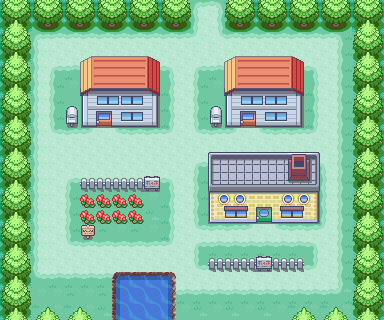
\includegraphics[width=2in]{PokemonPalletTown.png}
\end{center}
\caption{Pallet Town map from Pok\'{e}mon\cite{firered}} 
\label{fig:pokemon}
\end{figure}

\begin{table}
\label{table:symbols}
\caption{Symbols Names and the Hand drawn equivalents}
\begin{center}
\begin{tabular}{llll}
Water & 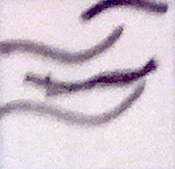
\includegraphics[width=.5in]{water.png} &
Grass & 
\includegraphics[width=.5in]{grass.png} \\
Rock & 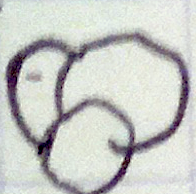
\includegraphics[width=.5in]{rocks.png} &
Tree & 
\includegraphics[width=.5in]{tree.png} \\
Dirt & 
\includegraphics[width=.5in]{dirt.png} &
Sand & 
\includegraphics[width=.5in]{sand.png} \\
\end{tabular}
\end{center}
\end{table}

We have created 6 symbols to be used to recreate maps for a popular video game
Pok\'{e}mon to ensure that our data set is sampled from a well defined distribution.
An example map from the game is shown in Figure \ref{fig:pokemon}. There is a sample
of the the symbols names and the hand drawn equivalents in Table \ref{table:symbols}.




\subsection{Preprocessing}
\label{process:preprocessing}

\begin{figure}[h]
    \begin{center}
    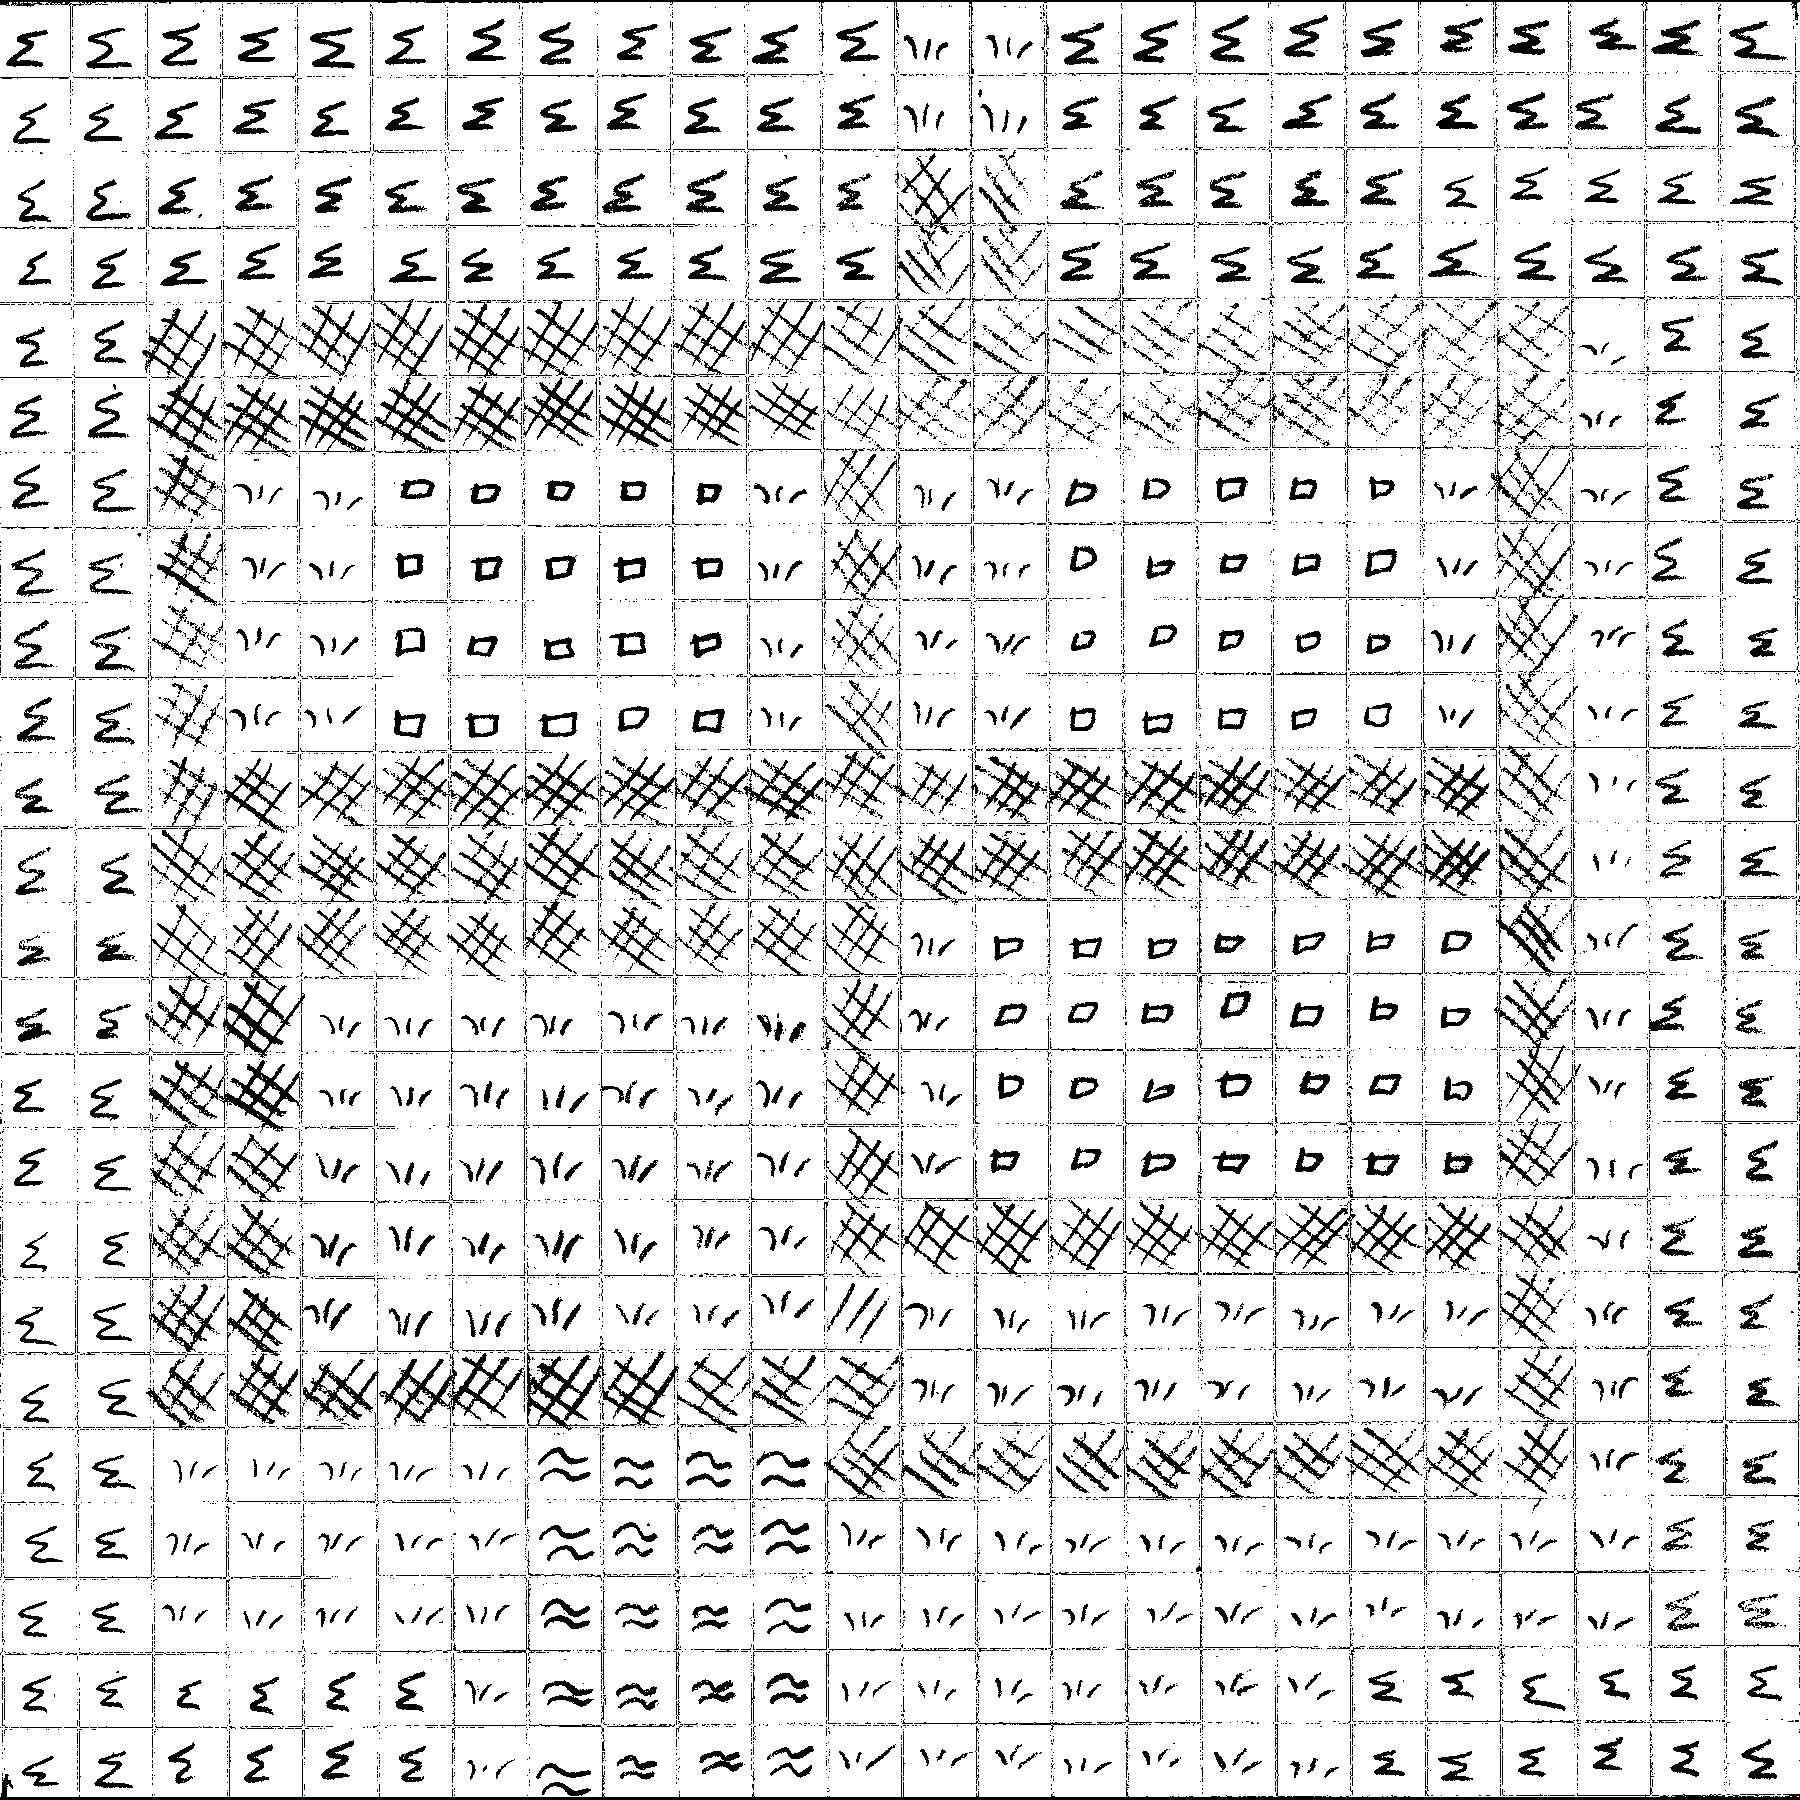
\includegraphics[width=7.5cm, height=7.5cm]{preprocessing-initial}
    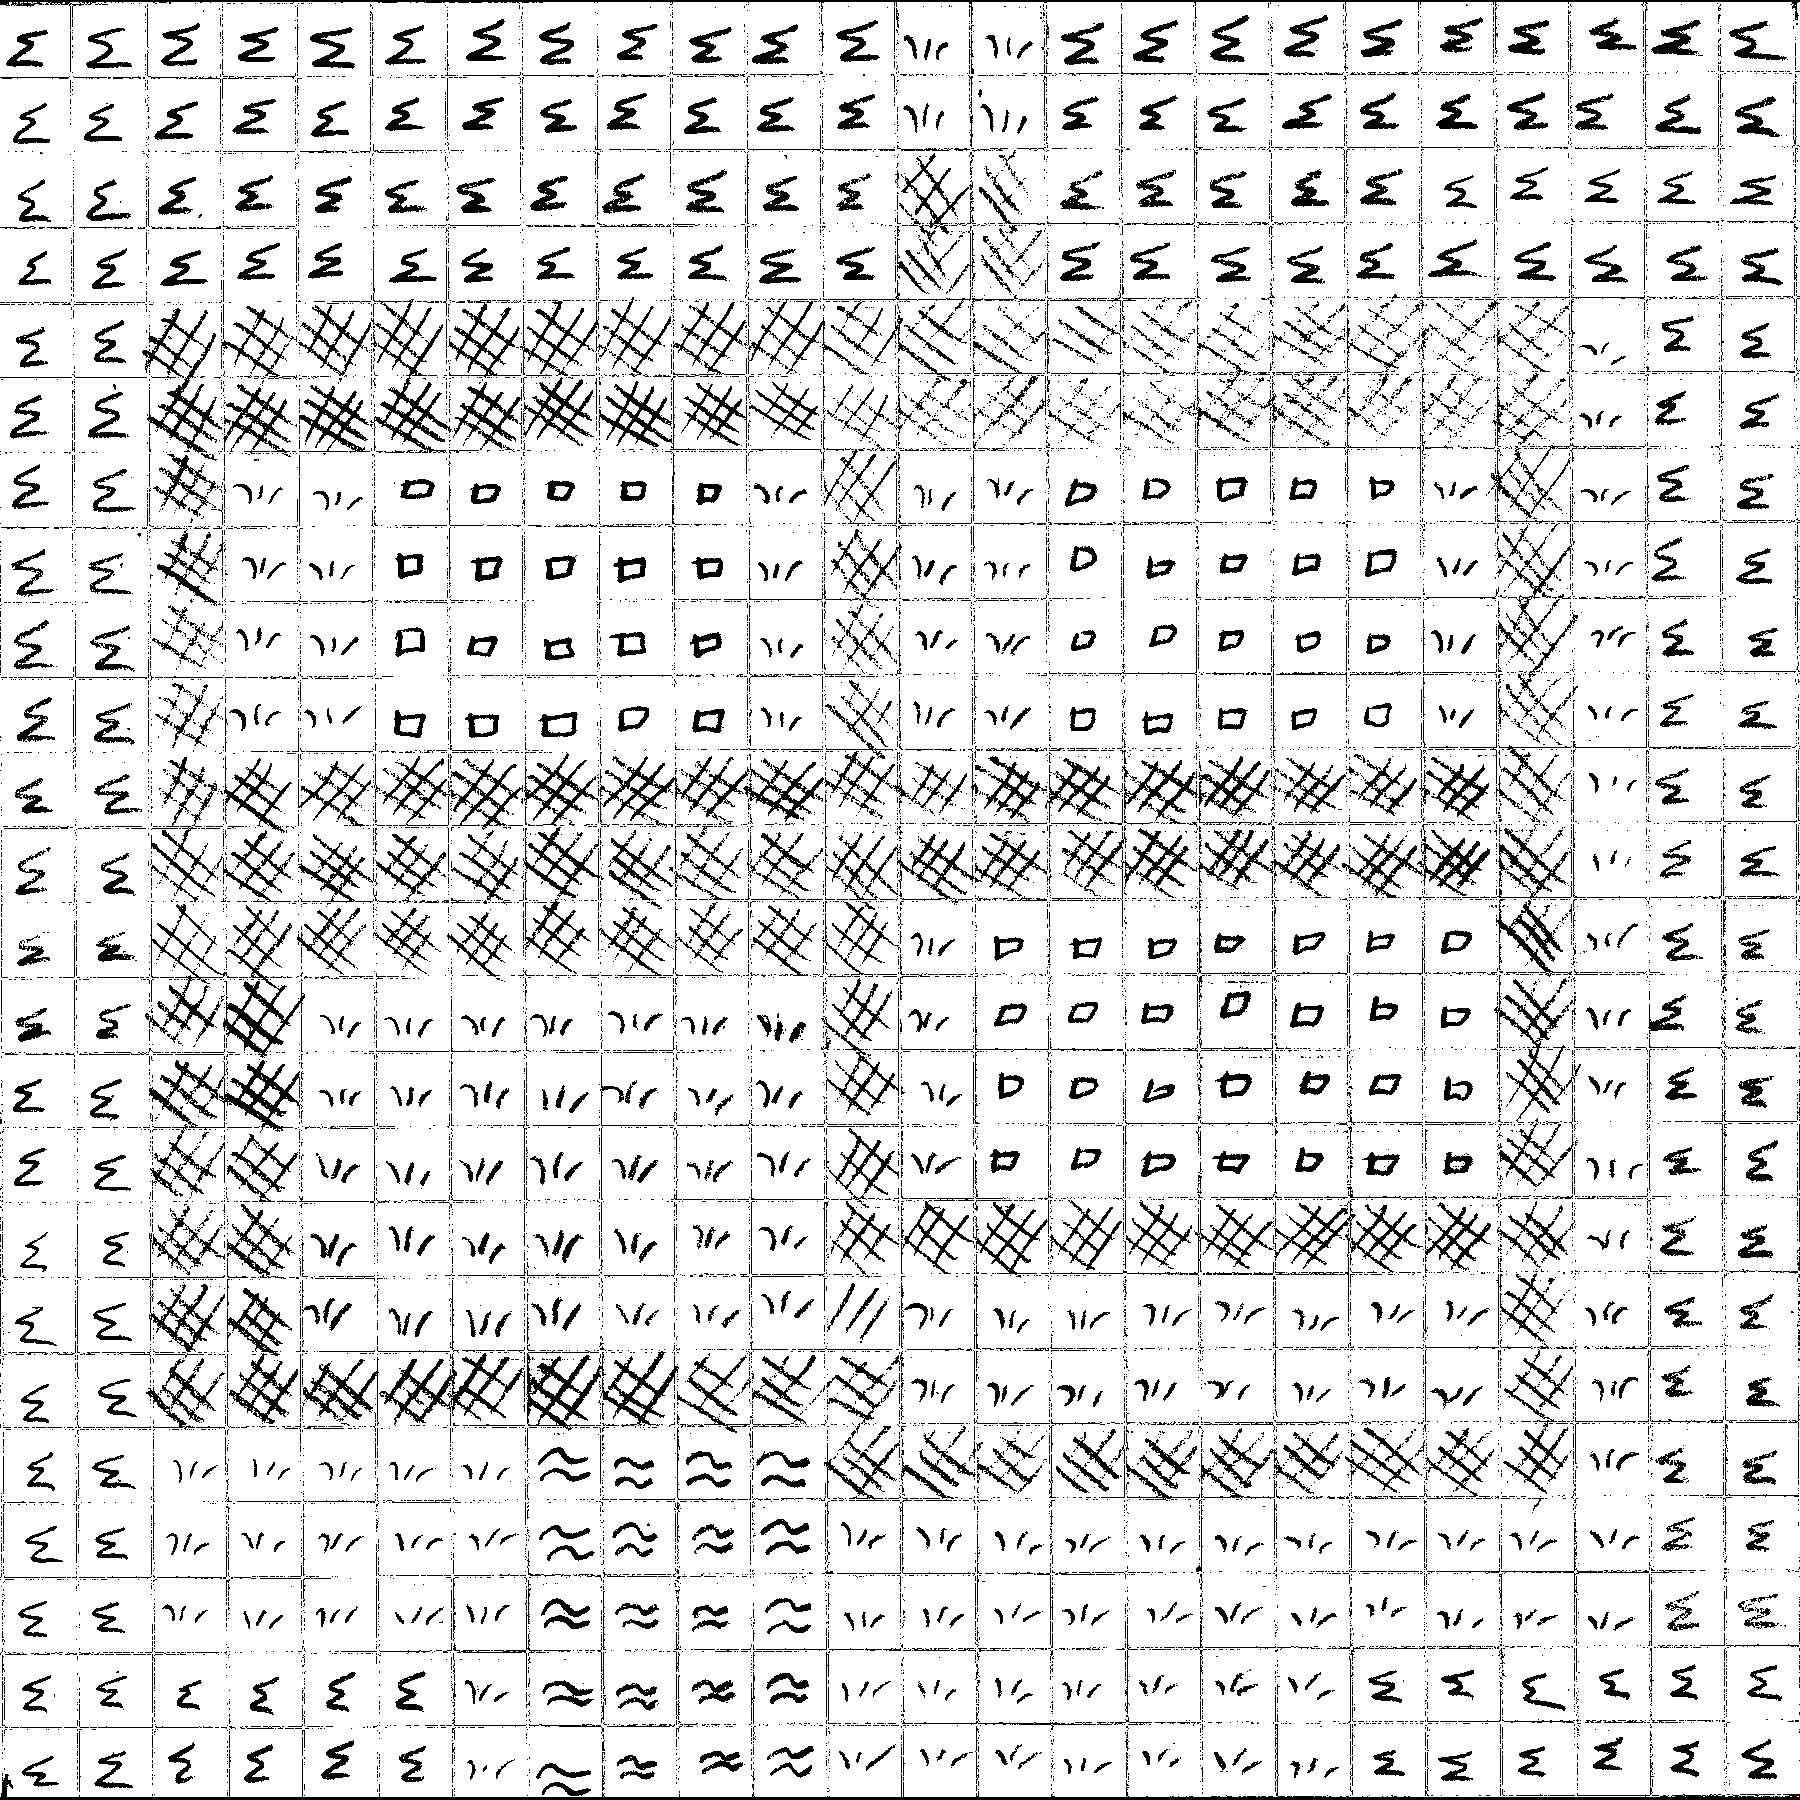
\includegraphics[width=7.5cm, height=7.5cm]{preprocessing-final}
    \label{figure:preprocess}
    \caption{Image before and after preprocessing. Note the increased contrast and faint grid lines}
    \end{center}
\end{figure}

Before analysis, the data must be preproccessed in order to standardize image
properties and reduce the risk of errors in classififcation. A collection of
scripts are run on each of the maps prior to classification to rotate, scale,
and remove the blue lines using colour filter masks.  Colour information is
removed from the images by converting them to black and white. Each cell is
scaled to a standard 75 by 75 pixels and seperated from the map such that each
cell contains a single symbol.  The results of preprocessing are shown in
Figure \ref{figure:preprocess}



\subsection{Feature-Based Approach}
\label{process:featurebased}

Feature based classification, as the name suggests, involves the classification of unknown cells through the use of geometric information regarding the shape and distribution of points from its contained physical symbol. To perform this task a collection of convolution filters were applied to each of the preprocessed cells. This was followed by statistical analysis on the distribution of black pixels in each of the of the $x$ and $y$ dimensions. These convolution filters are used to transform an image into another image which may make certain attributes, such as edges, more prominent.  For example, the convolution filter, $F_{blur}$ is a mean blur. The convolution filter transforms the image by replacing each pixel with a new filtered pixel. The new pixel is created by multiplying the surrounding values by those in the convolution filter and summing the result. This sum is the new value for the pixel. Each convolution filter consists of a matrix of odd size containing relevant coefficients to the feature that is being tested. In total nine filters were used, each extracting a different feature. 

\[ F_{blur} = \left[
\begin{array}{ccc}
1/16 & 2/16 & 1/16 \\
2/16 & 4/16 & 2/16 \\
1/16 & 2/16 & 1/16
\end{array}\right]
\]

\begin{figure}[h] \[
\begin{array}{lcr}
\begin{array}{ccccc}
\ddots & \vdots & \vdots & \vdots & \iddots \\
\ldots & 64 & 64 & 32 & \ldots \\
\ldots & 32 & \fbox{32} & 128 & \ldots \\
\ldots & 32 & 16 & 32 & \ldots \\
\iddots & \vdots & \vdots & \vdots & \ddots \\
\end{array} &
\begin{array}{c}
64F_{11} + 64F_{12} + 32F_{13} \\
+ 32F_{21} + 32F_{22} + 128F_{23} \\
+ 32F_{31} + 16F_{32} + 32F_{32} \\
\end{array} &
\begin{array}{ccccc}
\ddots & \vdots & \iddots \\
\ldots &  \fbox{48}  & \ldots \\
\iddots & \vdots & \ddots \\
\end{array}
\end{array} \]
\caption{Applying the convolution filter to the centred pixel area}
\label{figure:convolution}
\end{figure}

A filtered image is created as the result of the convolution matrix being
applied to each pixel. Figure \ref{figure:convolution} shows the filter being
applied to a single pixel. The filtering process repeats for each pixel until
all pixels have been replaced and resulting image has a luminance matrix,
which we will call $A$.

\[A = \left [
    \begin{array}{r r r r}
        a_{00} & a_{10} & \cdots & a_{n0} \\
        a_{01} & a_{11} & \cdots & a_{n1}\\
        \vdots  & \vdots  & \ddots & \vdots\\
        a_{0m} & a_{1m} & \cdots & a_{nm}\\
    \end{array}
\right ] \]

We define $x$ and $y$ to be the row and column sum functions.

\[
x(i) = \sum_{j}{A_{i,j}} \quad
y(j) = \sum_{i}{A_{i,j}}
\]

Next we record the means and standard deviations: $\mu_x, \mu_y, \sigma_x,
\sigma_y$ as the feature set for this filter. Then we apply another
filter, either on this filtered image or, on the original image and record
statistics on these as well.



\subsection{Gold Comparison Approach}


\begin{figure}[h]
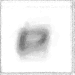
\includegraphics{building-mean}
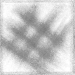
\includegraphics{dirt-mean}

\includegraphics{forest-mean}
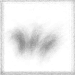
\includegraphics{grass-mean}
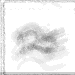
\includegraphics{water-mean}
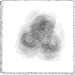
\includegraphics{rocks-mean}
\caption{The gold images created as the mean image of all examples of each symbol.
In order we have symbols representing buildings, dirt, forest, grass, water, and rocks.}
\label{figure:means}
\end{figure}

Similar to the feature-based approach, we define $x$ and $y$ to be the row and column sums
and calculate the mean and standard deviation of $x$ and $y$. To get the symbols to overlap we apply a
linear transformation to each pixel using the statistics gathered in each dimension.

\begin{equation} \label{eq:gold}
x^{\prime} = (x - \mu^{B}_{x}) \, \frac{\sigma^{G}_{x}}{\sigma^{C}_{x}} + \mu^{G}_{x} \quad
y^{\prime} = (y - \mu^{B}_{y}) \, \frac{\sigma^{G}_{y}}{\sigma^{C}_{y}} + \mu^{G}_{y}
\end{equation}

These new transformed pixels are placed into a new image $A$ which now overlaps with the
gold image $G$. We then compare the overlapping image $A$ to the gold standard image $G$ by taking the sum
of the squared difference at each pixel position. This gives us an error measure which we
record for each of the $k$ classes.

\[ \xi_{k}(A) = \sum_{i}\sum_{j}{(A_{ij} - G_{kij})^{2}} \]

The result is a vector of size $k$, the number of classes, with an error measure for the
comparison against the corresponding class. We then input this vector into WEKA along
with the correct answer for training purposes. We use a J48 decision tree with 10-fold
validation to train WEKA to classify using these error measures.

To create the gold images, we collected all the samples in our data set and 
created a mean gold image by overlapping all the smaples belonging to the same class,
the results can be seen in Figure \ref{figure:means}


\subsection{Proximity Approach}
\label{process:proximity}


The proximity classifier learns the patterns of symbols present in the data set
and then classifies any unknown symbols using the surrounding symbols and its
knowledge of the patterns and relationships of the symbols. Here we begin by
outlining the methodology used.  We want to classify the symbol $x$ at a given
position, as Figure~\ref{fig:neighbours} illustrates.

\begin{figure}[h]
\begin{center}
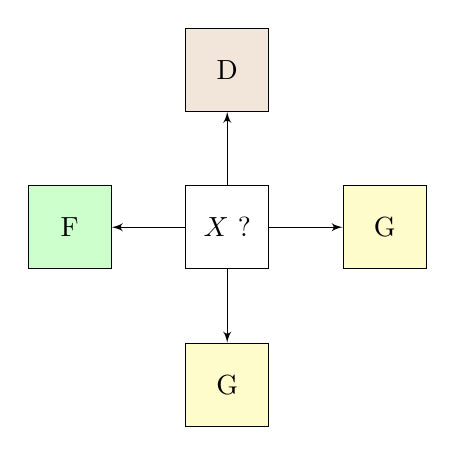
\begin{tikzpicture}[node distance=2cm, auto]
    \node[dcell](top){D};
    \node[ucell, below of=top](center){$X$~?};
    \node[fcell, left of=center](left){F};
    \node[gcell, right of=center](right){G};
    \node[gcell, below of=center](bottom){G};

    \path[line] (center)   -- node[right] {} (top);
    \path[line] (center)   -- node[above] {} (left);
    \path[line] (center)   -- node[above] {} (right);
    \path[line] (center)   -- node[right] {} (bottom);
\end{tikzpicture}
\end{center}
\caption{Cell 2,19 in Pallet Town, Note: $G$=grass, $D$=dirt, $F$=forest}
\label{fig:neighbours}
\end{figure}

To classify x, we first calculate the probability that $x$ belongs to each
class, $P(X)\quad X_i = P(x\!\in\! C_i)$.  The proximity classifier is given
the class of each symbol in the cardinal directions: north, south, east, and
west. Using this information, we restrict the probability calculation to only
consider the subspace where a symbol has the given classes neighbouring it.
Such a restriction is the conditional probability:

\[
P(X) = P(X|\,N\!=\!c_1,\,E\!=\!c_2,\,S\!=\!c_3,\,W\!=\!c_4)
\]

An example is shown in Figure~\ref{fig:conditionalprob}.

\begin{figure}[h]
\begin{center}
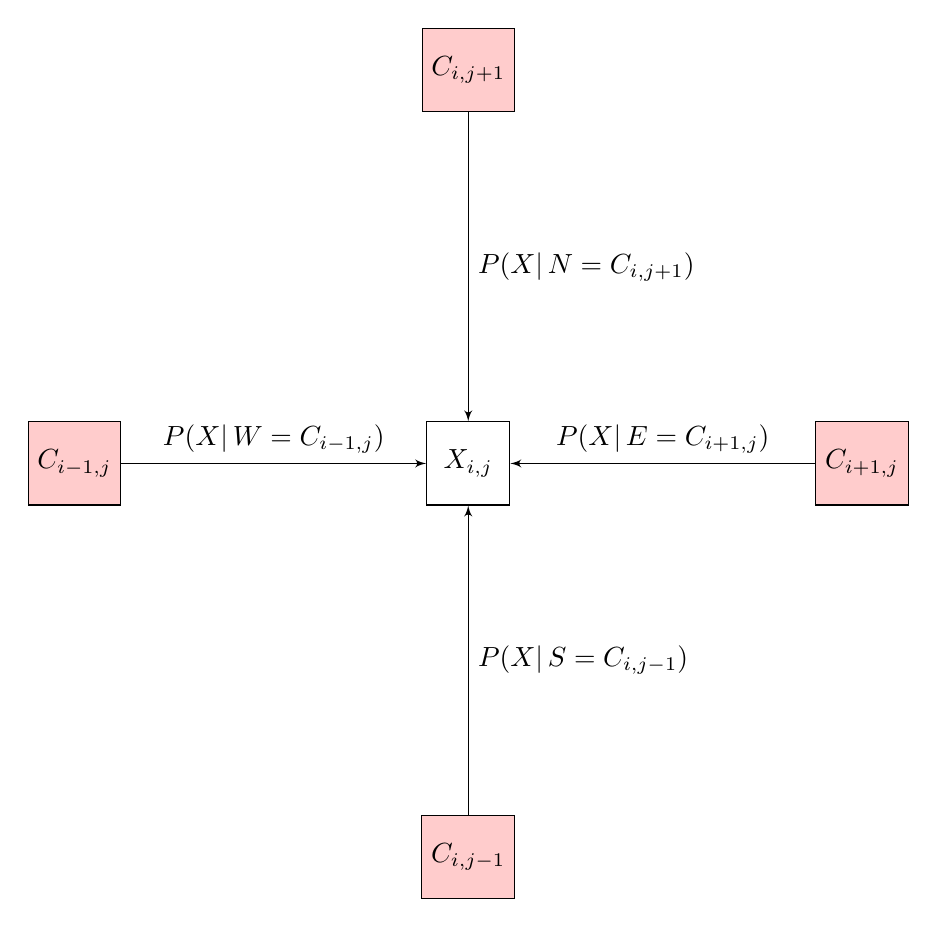
\begin{tikzpicture}[node distance = 5 cm, auto]
    \node[ccell](top){$C_{i,j+1}$};
    \node[ucell, below of=top](center){$X_{i,j}$};
    \node[ccell, left of=center](left){$C_{i-1,j}$};
    \node[ccell, right of=center](right){$C_{i+1,j}$};
    \node[ccell, below of=center](bottom){$C_{i,j-1}$};

    \path[line] (top)   -- node[right] {$P(X | \, N=C_{i,j+1})$} (center);

    \path[line] (left)  -- node[above] {$P(X | \, W=C_{i-1,j})$} (center);
    \path[line] (right) -- node[above] {$P(X | \, E=C_{i+1,j})$} (center);
    \path[line] (bottom) -- node[right] {$P(X | \, S=C_{i,j-1})$} (center);
\end{tikzpicture}
\end{center}
\caption{The conditional probability of the classes for $X_{i,j}$, given the neighbouring cells}
\label{fig:conditionalprob}
\end{figure}


In calculating probabilities, we can only approximate them using relative
frequencies collected from our sample data. For a set of $k$ classes, there are
$k^5$ possible combinations of neighbouring cells and the centre and too many
of these combinations occur rarely in our dataset to make confident
approximations of the true probabilities. To resolve this, we assume that the
conditional probabilities are independent in each direction. Under this
assumption, the calculation becomes much more reasonable for our small data set
since there are only $4k$ pieces of data to record for each symbol.  Our
resulting calculation becomes:

\begin{equation} \label{eq:prox}
P(X) \approx P(X|\,N\!=\!c_1)P(X|\,S\!=\!c_2)P(X|\,E\!=\!c_3)P(X|\,W\!=\!c_4)
\end{equation}

From the definition of conditional probability we have that for some class $c$ in
the direction $D$:
\[ P(X|\,D\!=\!c) = \frac{P(X \cap D\!=\!c)}{P(D=c)} \]

\begin{table}[h]
\label{table:relativefreq}
\begin{center}
\begin{tabular}{ l | r r r r r r }
              & $c_{B}$& $c_{D}$& $c_{EDGE}$& $c_{F}$& $c_{G}$& $c_{W}$ \\ 
              \hline
    north     & 0      & 0.1558 & 0.0519    & 0.0519 & 0.7403 & 0.0325\\
    east      & 0.0779 & 0.0974 & 0         & 0.1493 & 0.6428 & 0\\
    south     & 0      & 0.2403 & 0.0130    & 0.0065 & 0.7403 & 0\\
    west      & 0.0519 & 0.2273 & 0         & 0.0519 & 0.6428 & 0.0260\\
\end{tabular}
\caption{Probability of the neighbours for a grass cell in Pallet Town}
\end{center}
\end{table}


To calculate each of the conditional probabilities, we compute a table from the
samples recording $P(X\cap D\!=\!c)$ and $P(D\!=\!c)$ for each class  $c$, and
direction $D$ and example is given for a single class in
Table~\ref{table:relativefreq}.  We use the table to calculate the relative
conditional frequencies and, under the assumption of independence, we
approximate $P(X)$ using equation~\ref{eq:prox}.

Having the probability vector $P(X)$ we create an input file for WEKA.  This
file includes the probability vector, the neighbouring classes, and the class
of the symbol being classified for training. WEKA creates a decision tree which
is used to reduce the error in the probability calculation introduced under the
assumption of independence.



\subsection{Classifier Training}
\label{process:training}
Training was done using WEKA and 10-fold cross validation.
the proximity classifier was tested on a map it had never seen in training.

\section{Results}
\label{results}


\begin{tabular}{lrlrrr}
Algorithm & Samples & Feature Set & Success & Features & Tree nodes \\
\hline
Feature-Based   & 9888  & Single Filter & 76.32 &  32 & ? \\
Feature-Based   & 9888  & No Spatial    & 80.64 & 205 & 1131 \\
Feature-Based   & 9888  & Spatial       & 82.47 & 207 & 1005 \\
Proximity       & 13200 & Surrounding   & 93.78 &  11 & ? \\ 
Gold Comparison & 225   & Probabilities & 70.40 &   7 & ? \\
Gold Comparison & 225   & Probabilities & 83.33 &   7 & ? \\
\end{tabular}



\section{Conclusions}
\label{conclusions}

Each of our classification methods has its strengths and weaknesses.  The
feature based method is able to recognize arbitrary features and is very easy
to extend by adding new filters.  The proximity method works extremely well
with the set of maps we chose because there are many common patterns in their
composition.  However, to detect these patterns in a data set the proximity
classifier needs an accurate representation of the map. This method has the
added benefit of having its output be the same as its input, which means it can
improve its output iteratively.  The gold comparison method is able to classify
symbols fairly well. However, this method requires gold images as input and the
number of features in the output is dependent on the number of gold images
(which makes generalization more difficult).



\section{Further Work}
\label{further work}


Future expansion of this design is possible and we believe the results are
encouraging.  After assessing the results, we have identified various aspects
of our current design that can be changed to improve the functionality and
classification results. For example, we would like to use all the methods
presented here in conjunction to improve the accuracy and the robustness of the
system.  One such system, could run the gold comparison method to get a rough
approximation of the layout of the symbols and then use the proximity method to
improve the confidence in the results. 

Improving on the individual methods is also possible as the feature based
classification may see improvement from considering other transformations of
the pixels when calculating statistics, such as the distance from the centre
which is especially useful for symmetric shapes. 

Another improvement that we would have like to make is to limit the
region of the cell which the feature based method analyses.  By only taking
statistics on these smaller sections of the images we could eliminate areas of
the image that are largely noise, such as the edges of the cell.

The gold comparison method could use ``ideal'' gold images rather than mean
gold images and we suspect that the performance of the gold method could be
improved by using carefully selected images that better illustrate the intended
shape of the character. Also, adding more than one ``gold'' symbol for each
class may allow for more variations than the mean of each variation.

Given the strength of the patterns and relationships found by the proximity
statistics, the extensibility of the feature based method, and the accuracy of
the gold image classifier, we believe the results show promise in a hybrid
approach of the proposed methods to create an accurate, robust, and extensible
classification system.



\section{References}
\label{references}


\bibliographystyle{plain}
\bibliography{report}


\end{document}

